\documentclass[10pt]{article}
\usepackage[margin=0.72in]{geometry}
\usepackage{amsmath,amssymb}
\usepackage{booktabs,longtable,tabularx,array}
\usepackage{graphicx}
\usepackage{xcolor}
\usepackage{hyperref}
\usepackage{enumitem}
\usepackage{microtype}
\usepackage{fancyhdr}
\usepackage{caption}
\definecolor{navy}{HTML}{17365D}
\definecolor{blue}{HTML}{2878B5}
\definecolor{red}{HTML}{A23B3B}
\definecolor{light}{HTML}{F2F5F8}
\hypersetup{colorlinks=true,linkcolor=navy,urlcolor=blue,citecolor=navy}
\setlist{nosep,leftmargin=1.35em}
\setlength{\parindent}{0pt}
\setlength{\parskip}{4pt}
\captionsetup{font=small,labelfont=bf}
\pagestyle{fancy}
\fancyhf{}
\lhead{\sffamily\small Gaussian Data Regression}
\rhead{\sffamily\small Technical report and data audit}
\cfoot{\thepage}
\newcommand{\code}[1]{\texttt{#1}}
\newcommand{\evidence}[1]{\textcolor{navy}{\footnotesize\textsf{Evidence: #1}}}
\newcommand{\paperquote}[2]{%
  \begin{quote}\small\textbf{Paper [#1] says:} ``#2''\end{quote}}
\newcommand{\localquote}[2]{%
  \begin{quote}\small\textbf{Local source #1 says:} ``#2''\end{quote}}
\newcommand{\tvd}{\mathrm{TVD}}
\newcolumntype{Y}{>{\raggedright\arraybackslash}X}

\begin{document}

\begin{titlepage}
\color{navy}
\vspace*{1.0cm}
{\sffamily\bfseries\fontsize{25}{29}\selectfont
Gaussian-Data-Regression Error Mitigation\\[4pt]
for a Hybrid Qubit--Qumode VQE\par}
\vspace{0.45cm}
{\sffamily\Large Technical documentation, literature traceability, and independent data audit\par}
\vspace{0.8cm}
\color{black}
\begin{tabular}{@{}ll@{}}
Repository area & \path{Error_mitigation/}\\
Frozen experiment & mixed p-spin instance H000\\
Report date & 8 September 2026\\
Primary matrix & 108 cells; 8,192 shots; 40 training twins per cell\\
Headline method & official \code{gdr\_param} in \path{out/results.json}\\
\end{tabular}
\vfill
\colorbox{light}{\parbox{0.94\textwidth}{
\textbf{Executive result.}
Using only the official stored \code{gdr\_param} records gives mean TVD
$0.3312\rightarrow0.1850$ and median TVD $0.2850\rightarrow0.1273$.
TVD improves in 93 of 108 cells and worsens in 15, almost all ECD/random cells at
$\kappa\tau\ge0.03$. Absolute energy error improves in 64 of 108 cells and worsens
in 44, so TVD success must not be misreported as universal observable-level success.

\evidence{Local data D1; independently recomputed by C7, output D6.}
}}
\vfill
{\small This report distinguishes three kinds of evidence: scholarly literature quotations [1]--[10],
repository implementation C1--C7, and stored experiment data D1--D6. Local experimental values are
not attributed to external papers.}
\end{titlepage}

\tableofcontents
\newpage

\section{Direct answers}

\subsection{What is a Gaussian gate?}

\textbf{Definition.} For $m$ bosonic modes, collect quadratures as
$\hat{x}=(\hat{q}_1,\hat{p}_1,\ldots,\hat{q}_m,\hat{p}_m)^T$.
A state is Gaussian when its Wigner function (equivalently, its characteristic function) is a
multivariate Gaussian. It is therefore completely specified by the first moment
$\bar{x}=\langle\hat{x}\rangle$ and covariance matrix $V$. A Gaussian operation maps Gaussian states
to Gaussian states. A Gaussian unitary is generated by a Hamiltonian no higher than quadratic in the
field operators, and acts as
\[
  \bar{x}\mapsto S\bar{x}+d,\qquad V\mapsto SVS^T,
\]
where $S$ is symplectic.

\paperquote{1}{By definition, these are bosonic states whose Wigner representation
(\(\chi\) or \(W\)) is Gaussian.}
\paperquote{1}{Gaussian unitaries are generated ... from Hamiltonians \(\hat H\) which are
second-order polynomials in the field operators.}
\paperquote{1}{Thus the action of a Gaussian unitary ... over a Gaussian state
\(\hat\rho(\bar{x},V)\) is completely characterized by Eq.~(25).}

\textbf{Why the name?} It is literal: the phase-space probability-like representation has the
Gaussian exponential form, and quadratic Hamiltonians preserve that form. Common Gaussian gates are
displacement, phase rotation, single- and two-mode squeezing, and beam splitters. Kerr, cubic-phase,
and a general number-dependent SNAP phase are non-Gaussian.

\textbf{Important scope warning.} ``Gaussian gates are easy'' is incomplete. Efficient covariance
tracking applies to Gaussian states, Gaussian transformations, and compatible Gaussian measurements
(for example homodyne/heterodyne). Photon-number measurement can make an otherwise Gaussian optical
circuit classically hard: Gaussian boson sampling evaluates hafnians.

\paperquote{4}{We relate the probability to measure specific photon patterns from a general Gaussian
state in the Fock basis to a matrix function called the hafnian ... [and] design Gaussian Boson
sampling, a \#P hard problem.}
This is an exact-output hardness statement. Paper [4] leaves the corresponding approximate-sampling
claim conditional on hafnian and anticoncentration conjectures; this report does not present it as
an unconditional theorem.

\subsection{Why, and how much, easier is classical simulation?}

\begin{table}[h]
\centering\small
\begin{tabularx}{\textwidth}{@{}p{0.20\textwidth}p{0.29\textwidth}Y@{}}
\toprule
Regime & Stored description / representative cost & What can safely be concluded\\
\midrule
Gaussian state, Gaussian gates &
$2m$ means plus a $2m\times2m$ covariance: $O(m^2)$ memory.
Dense covariance updates are at most $O(m^3)$ arithmetic per generic dense transform; local gates
can be cheaper. &
Polynomial in mode count, independent of any per-mode Fock cutoff. The $O(m^3)$ statement is a
dense-linear-algebra bound derived from Eq.~(25) of [1], not a claim of optimality.\\
\addlinespace
CV stabilizer formulation &
Paper [2] tracks $4m^2$ real numbers for finitely squeezed inputs. &
Paper-supported polynomial-size representation. Paper [2] proves efficient simulation for its listed
inputs, quadratic gates, quadrature measurements, finite loss, and feed-forward.\\
\addlinespace
Generic cutoff statevector &
With local cutoff $D$, a ket contains $D^m$ complex amplitudes; a density matrix contains $D^{2m}$
complex entries. &
Exponential in mode count at fixed $D$. This is dimension counting, not a lower bound for every
non-Gaussian circuit and not the algorithm used for the easy twins.\\
\addlinespace
Non-Gaussian state as $\chi$ Gaussian terms &
Exact strong simulation $O(s\chi^2m^3)$ for $s$ Gaussian unitaries in the model of [5];
an approximate bounded-energy algorithm is linear in $\chi$ with additional accuracy/energy factors. &
Cost is controlled by a non-Gaussian resource measure, not by a universal ``non-Gaussian =
exponential'' rule. If a particular decomposition doubles $\chi$ at each of $t$ injections, then
$\chi=2^t$ gives a $4^t$ factor for the exact algorithm; that conditional statement is not universal.\\
\bottomrule
\end{tabularx}
\caption{Classical simulation scaling. Symbols: $m$ modes, cutoff $D$, $s$ Gaussian operations,
Gaussian rank $\chi$, and number of non-Gaussian injections $t$.}
\end{table}

\paperquote{2}{A classical simulation requires following the evolution of \(4n^2\) numbers.}
\paperquote{2}{As only the operations of addition and multiplication are required, the
discretization error can be kept bounded with a polynomial cost to efficiency.}
\paperquote{5}{[The] exact simulation algorithm [has] runtime ... quadratic in the number of terms in
the superposition. We also present a faster approximate randomized algorithm whose runtime is linear
in this number.}
\paperquote{5}{[It] computes the value \(p(\alpha)\) exactly in time
\(O(s\chi^2n^3)\).}

\textbf{Non-Gaussian gates are not assigned one cost.} A non-Gaussian gate is valuable precisely
because it leaves the covariance-only class and enables universal CV computation, but simulation
complexity depends on energy, cutoff, gate structure, desired observable, approximation error, and
the available decomposition.

\paperquote{3}{Translations, phase shifts, squeezers, and beam splitters, combined with some
nonlinear operation such as a Kerr nonlinearity, suffice to enact to an arbitrary degree of accuracy
Hamiltonian operators that are arbitrary polynomials over a set of continuous variables.}

\textbf{Audit note on this folder.} The README phrase ``Gaussian rank \(2^t\)'' for twins with
\code{t\_free} non-Gaussian gates is not established by the implementation: C2 records
\code{t\_free}, but does not construct or certify a minimum Gaussian decomposition. Treat
\(2^t\) as motivation or a loose branching picture, not a measured rank or proved runtime.

\subsection{Why the twins in this project are easy}

The target is hybrid: one qubit plus two bosonic modes, measured as a
$|q,n_1,n_2\rangle$ histogram. ``Gaussian'' applies to the bosonic modes; the ancilla handling must
also avoid creating unresolved superpositions.

\begin{itemize}
\item \textbf{ECD twin.} Each ancilla angle is snapped to $0$ or $\pi$. The ancilla therefore stays
in a computational-basis branch; each ECD becomes an unconditional displacement (plus a possible
bit flip). Starting from vacuum, the output is
$|q\rangle|\alpha_1\rangle|\alpha_2\rangle$.
\item \textbf{SNAP twin.} Each phase list $\theta_n$ is replaced by its least-squares affine fit
$bn$ with $\theta_0=0$. Since $\exp(i b\hat n)$ is a phase rotation, the remaining circuit is
displacements and rotations.
\item \textbf{Analytic histogram.} For a product coherent state,
$P(q,n_1,n_2)=\delta_{q,q_0}\prod_j e^{-|\alpha_j|^2}|\alpha_j|^{2n_j}/n_j!$
before finite-cutoff corrections. The code also performs exact truncated one-mode propagation and
asserts it against the full statevector at TVD below $10^{-6}$.
\end{itemize}
\evidence{C2 (\path{twins.py}); D1 reports product-state TVD maximum
\(1.13\times10^{-15}\) for the frozen baseline. These are local validation values, not literature
claims.}

\section{How error mitigation is performed}

\subsection{Implemented workflow, step by step}

This report uses one method, \code{gdr\_param}, on the official frozen 108-cell matrix.
Later research variants (\code{gdr\_damped}, \code{gdr\_floor}, \code{gdr\_select}, and
span-twin replays) are not used for any headline number or figure.

\begin{enumerate}[label=\textbf{Step \arabic*.},leftmargin=3.6em,itemsep=5pt]
\item \textbf{Fix the target and metric.} Load H000, run ECD at depth 5 or SNAP at depth 2, and define
the ideal $|q,n_1,n_2\rangle$ distribution. Compare histograms with
\(\tvd(p,q)=\frac12\sum_i|p_i-q_i|\); also retain Hellinger distance and observable errors.
\evidence{C1, C4; D1.}

\item \textbf{Choose a matched training design.} Use 40 twins at the same circuit depth and gate
count. The official matrix samples amplitude scales from the default mix $U(0.5,1)$.
Thirty twins are fully Gaussian and ten retain two original gates.
\evidence{C2; D1.}

\item \textbf{Compute ideal twin outputs classically.} For fully Gaussian twins, use product
one-mode propagation; validate against the full simulator. Twins retaining original gates use the
full statevector path. This mirrors CDR's use of target-like circuits whose exact answers remain
classically accessible.
\paperquote{6}{The training data are obtained from quantum circuits composed largely of Clifford
gates ... and hence these circuits are efficiently classically simulable. Next we fit the training
data with a model, and finally we use the fitted model to predict the noise-free observable.}

\item \textbf{Run the same noisy channel and readout on target and twins.} The matrix sweeps three
circuit-noise families, $\kappa\tau\in\{0.003,0.03,0.1\}$, and ideal/realistic/strong readout.
Each stored cell uses 8,192 shots. \evidence{C3; D1.}

\item \textbf{Fit a structured transfer model jointly.} Fit 11 bounded parameters by multinomial
maximum likelihood: two transmissions, two thermal occupations, shared down/up hops and leak, two
qubit readout probabilities, and two Fock nearest-neighbor readout probabilities. The model factors
as $M=C_q\otimes C_1\otimes C_2$. \evidence{C5.}

\item \textbf{Unfold the target histogram.} Apply Richardson--Lucy iterations to
$q_{\mathrm{obs}}\approx Mp$, preserving non-negativity and normalization.
This unfold, with the fitted parametric kernel, is \code{gdr\_param}.
\paperquote{10}{The technique ... conserves the constraints on frequency distributions
(i.e., normalization and non-negativeness) and, at each iteration, increases the likelihood of the
observed sample.}

\item \textbf{Handle readout before ZNE when ZNE is reported.} Readout is not changed when idle
noise is stretched. Therefore invert calibrated readout at each scale and only then extrapolate
to zero circuit noise. ZNE is a stored comparator in D1, not the headline method.
\paperquote{8}{The first method, extrapolation to the zero noise limit, subsequently cancels powers
of the noise perturbations by an application of Richardson's deferred approach to the limit.}

\item \textbf{Report diagnostics and caveats.} Store TVD, Hellinger distance, energy error, ground
state probability error, fitted versus true parameters, and oracle residuals. Never infer observable
accuracy from TVD alone. \evidence{C1, C4; D6.}
\end{enumerate}

\subsection{Relation to prior methods}

This is a histogram-level, structured extension of Clifford Data Regression: target-like Gaussian
twins replace target-like Clifford circuits, and a transfer matrix replaces scalar linear
regression. The project's 40 twins are a local engineering choice. They must not be justified by
CDR's unrelated empirical count without qualification.

\paperquote{6}{In the case of our QAOA implementation we observe that 60--80 training circuits and
8192 shots per expectation value estimation are enough to obtain an order of magnitude improvement
for ... \(Q=8\)--64 and ... \(p=1\)--24.}

Paper [6] therefore supports the \emph{training-data concept} and reports its own numerical regime;
it does not prove that 40 twins are sufficient here. The project's adequacy evidence is the
full-matrix \code{gdr\_param} performance in D1 and D6.

Readout-only inversion is also literature grounded:
\paperquote{7}{If the measurement device is affected only by an invertible classical noise, it is
possible to correct the outcome statistics of future experiments performed on the same device.}
The nearest-neighbor Fock readout values here are simulated assumptions. Paper [9] provides a useful
experimental scale but uses a more detailed hidden Markov model:
\paperquote{9}{The mitigation improves the average total variation distance error of Fock states
from 13.5\% to 1.1\%.}
This quote supports the README's comparison scale; it does not validate this folder's static,
uncorrelated confusion matrix.

\section{Independent analysis of mitigation quality}

\subsection{Analysis protocol}

No existing PNG was reused. Script C7 reads the official 108-cell matrix D1 and takes
\code{gdr\_param} for every cell. It then independently aggregates the stored per-cell metrics
and creates all six figures below, including two stored-case histograms reconstructed from the
D1 \code{cases} payload. The exact machine-readable output is D6. Later research
JSON under \path{out_research/} is not mixed into this scoreboard.

\subsection{Distribution-level result}

\begin{figure}[h]
\centering
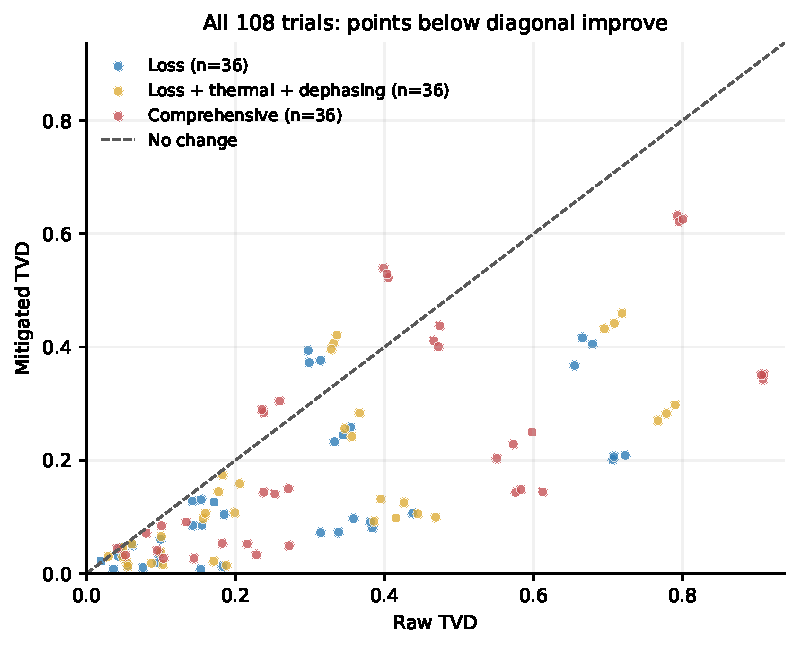
\includegraphics[width=0.65\textwidth]{report_assets/figures/paired_tvd.pdf}
\caption{Each point is one stored cell. Points below the diagonal improve TVD.
Twelve ECD/random high-noise cells and three mild SNAP/random ideal-readout cells lie above it.
Source: D1; reconstruction C7.}
\end{figure}

\begin{table}[h]
\centering\small
\begin{tabular}{@{}lrrr@{}}
\toprule
Metric & Raw & \code{gdr\_param} & Change / count\\
\midrule
Mean TVD & 0.3312 & 0.1850 & 44.2\% reduction of pooled mean\\
Median TVD & 0.2850 & 0.1273 & cellwise median reduction 42.0\%\\
Cells strictly improving TVD & \multicolumn{2}{c}{93 / 108} & 86.1\%\\
Cells with TVD regression & \multicolumn{2}{c}{15 / 108} & 13.9\%\\
\bottomrule
\end{tabular}
\caption{Independent aggregate. Every number is computed from local stored data D1 by C7,
not taken from an existing figure.}
\end{table}

The reduction is not uniform. Pooled mean TVD falls by 49.3\% for pure loss, 46.4\% for
loss+thermal+dephasing, and 38.8\% for comprehensive noise. By noise strength, pooled reductions are
64.8\%, 57.1\%, and 33.0\% at $\kappa\tau=0.003$, $0.03$, and $0.1$, respectively.
The 15 TVD regressions are concentrated on ECD/random cells at $\kappa\tau\ge0.03$, where the
parametric unfold over-corrects. Optimized cells improve in all 54 cases.
\evidence{D6; each family has 36 cells and each noise strength has 36 cells.}

\begin{figure}[!ht]
\centering
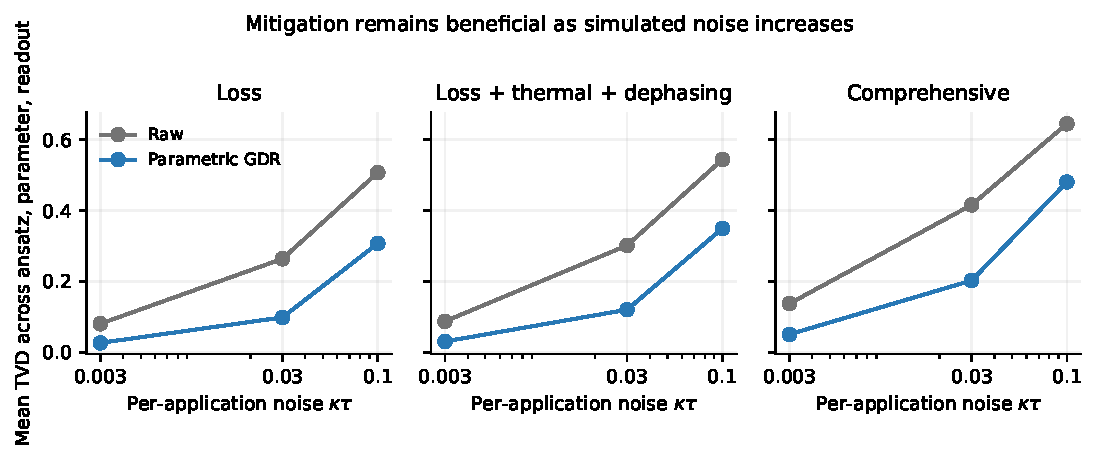
\includegraphics[width=0.96\textwidth]{report_assets/figures/tvd_by_noise.pdf}
\caption{Mean TVD across ansatz, parameter regime, and readout for each family/noise pair.
Lines summarize heterogenous cells; they are not statistical confidence intervals. Source D1,
computed by C7.}
\end{figure}

\begin{figure}[!ht]
\centering
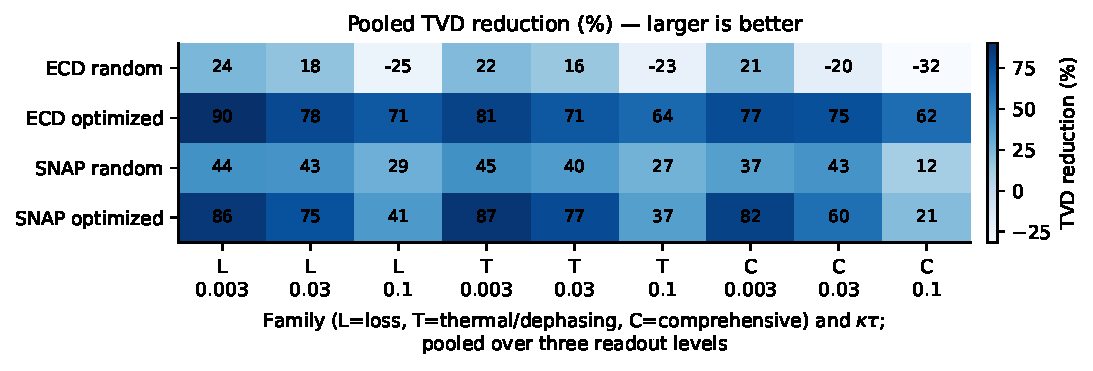
\includegraphics[width=0.98\textwidth]{report_assets/figures/improvement_heatmap.pdf}
\caption{Pooled TVD reduction over the three readout levels. Negative entries are the ECD/random
high-noise block, where \code{gdr\_param} over-corrects. Source D1, computed by C7.}
\end{figure}
\clearpage

Two stored cells make that TVD movement visible as histograms, one per ansatz, under the
same noise and readout. Both are optimized circuits at $\kappa\tau=0.03$ with strong readout
and loss+thermal+dephasing, the regime where the method is strongest rather than a low-noise
readout-only cleanup.

The SNAP cell has three resolved ideal peaks. The raw histogram is smeared, and
\code{gdr\_param} improves both TVD ($0.4687\rightarrow0.0994$) and absolute energy error
($1.719\rightarrow0.523$).

\begin{figure}[!ht]
\centering
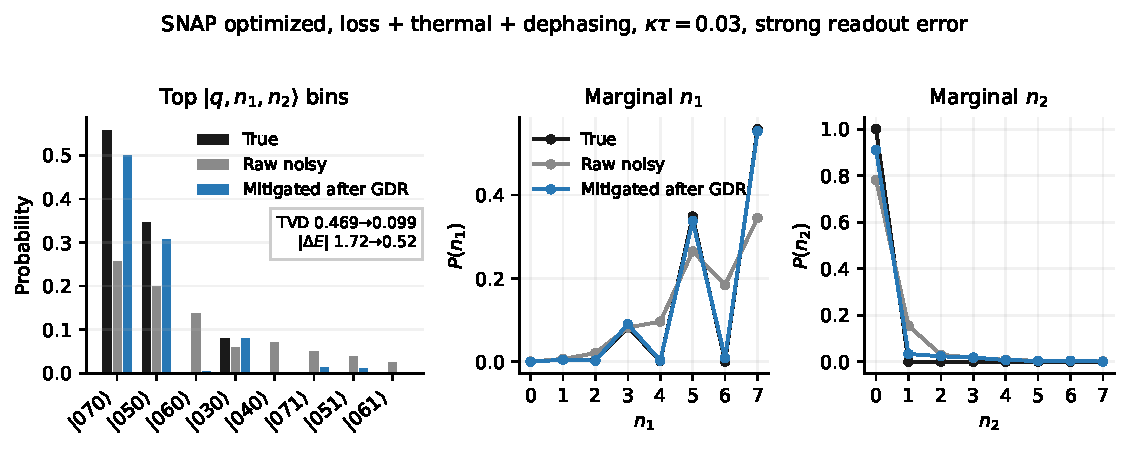
\includegraphics[width=\textwidth]{report_assets/figures/case_histogram_snap.pdf}
\caption{True, raw-noisy, and \code{gdr\_param} histograms for the official SNAP cell
(optimized; loss+thermal+dephasing; $\kappa\tau=0.03$; strong readout).
Left: joint probabilities on the largest $|q,n_1,n_2\rangle$ bins, including raw leakage
such as $|060\rangle$ and $|040\rangle$.
Centre: mode-1 Fock marginal $P(n_1)=\sum_{q,n_2}P(q,n_1,n_2)$.
Right: mode-2 Fock marginal $P(n_2)=\sum_{q,n_1}P(q,n_1,n_2)$.
Source D1 \code{cases}; reconstruction C7.}
\end{figure}

The matching ECD cell is a nearly pure $|070\rangle$ target. Photon loss and strong readout
move probability into $|060\rangle$ and $|170\rangle$; \code{gdr\_param} restores the peak
and improves both TVD ($0.4448\rightarrow0.1055$) and absolute energy error
($1.622\rightarrow0.542$).

\begin{figure}[!ht]
\centering
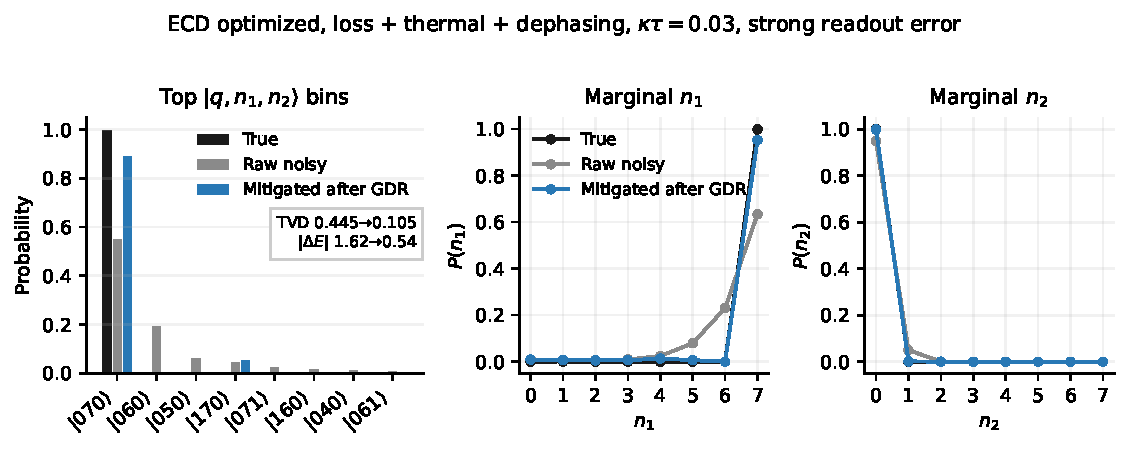
\includegraphics[width=\textwidth]{report_assets/figures/case_histogram_ecd.pdf}
\caption{True, raw-noisy, and \code{gdr\_param} histograms for the official ECD cell
(optimized; loss+thermal+dephasing; $\kappa\tau=0.03$; strong readout).
Left: joint probabilities on the largest $|q,n_1,n_2\rangle$ bins, including raw leakage
such as $|060\rangle$ and $|170\rangle$.
Centre: mode-1 Fock marginal $P(n_1)=\sum_{q,n_2}P(q,n_1,n_2)$.
Right: mode-2 Fock marginal $P(n_2)=\sum_{q,n_1}P(q,n_1,n_2)$.
Source D1 \code{cases}; reconstruction C7.}
\end{figure}
\clearpage

\subsection{Observable-level result and limitation}

Mean absolute energy error falls from $0.9349$ to $0.4876$, but the median rises from $0.2333$ to
$0.2794$. Cellwise energy error improves in 64 of 108 cells and worsens in 44 of 108.
This is not contradictory: TVD weights all histogram bins equally in probability mass, while the
energy applies problem-specific bin weights; finite-shot changes can improve one and worsen the
other. \evidence{D6.}

\begin{figure}[h]
\centering
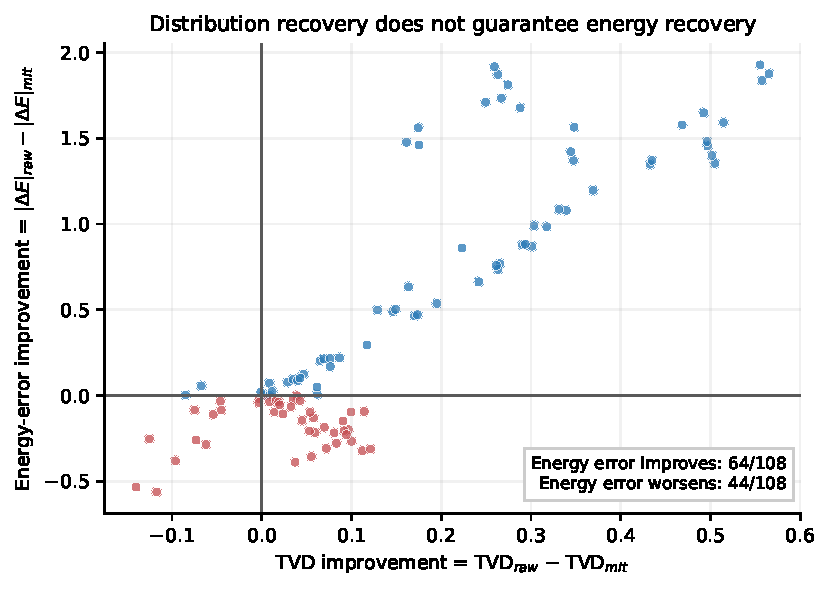
\includegraphics[width=0.67\textwidth]{report_assets/figures/energy_tradeoff.pdf}
\caption{Positive horizontal values improve TVD; positive vertical values improve absolute energy
error. Red points are the 44 cells where energy error worsens, including cells whose TVD also
regresses. Source D1, computed by C7.}
\end{figure}

\subsection{Uncertainty: what is and is not established}

The official 108-cell matrix contains one finite-shot realization per cell; variation across cells
is not a confidence interval. This report does not attach later span-twin bootstrap files to the
official \code{gdr\_param} scoreboard, because those resamples used a different twin design.

The 15 TVD regressions and 44 energy regressions are therefore exact counts on this stored draw,
not estimated rates with a standard error. They do not test hardware drift and do not provide a
multi-instance Hamiltonian confidence interval.

\section{What was done in the folder}

\begin{longtable}{@{}p{0.22\textwidth}p{0.72\textwidth}@{}}
\toprule
Area & Role\\
\midrule
\endhead
\path{metrics.py} & Normalizes histograms and computes TVD, Hellinger distance, absolute energy
error, ground-state-probability error, and Gibbs-objective error.\\
\path{noise_models.py} & Defines pure loss, thermal+dephasing, and comprehensive circuit-noise
families; three final-readout confusion settings; and circuit-noise scaling for ZNE.\\
\path{twins.py} & Constructs ECD and SNAP twins, tracks coherent amplitudes, computes product
histograms, validates against statevectors, and defines default/span twin plans.\\
\path{mitigation.py} & Implements transfer kernels, multinomial fitting, Richardson--Lucy and NNLS
unfolding, readout correction, damping/selection, residual ablations, scalar CDR, and ZNE variants.\\
\path{run_mitigation_experiment.py} & Official baseline driver; writes the frozen \path{out/}
artifacts used by this report.\\
\path{run_ablation.py} & Research driver with physics caching; later method variants live under
\path{out_research/} and are not used here.\\
\path{out/} & Official frozen matrix: 108 cells, including \code{gdr\_param}, summaries, optimized
parameters, and diagnostic plots.\\
\path{out_research/} & Later ablations and alternative selectors. Kept on disk but excluded from
the headline scoreboard.\\
\path{report_assets/} & Reproducible analysis script, machine-readable aggregate, and figures created
for this report.\\
\bottomrule
\end{longtable}

\clearpage
\section{Noise model and interpretation}

\begin{table}[h]
\centering\small
\begin{tabularx}{\textwidth}{@{}p{0.20\textwidth}YY@{}}
\toprule
Family & Local implementation & Main interpretation limit\\
\midrule
Loss & Pure photon loss after each UER/SNAP layer. & An end-of-circuit binomial kernel is exact only
when interleaving can be ignored.\\
Loss + thermal + dephasing & Thermal occupation $n_{\rm th}=0.05$ and
$\kappa_\phi\tau=0.5\kappa\tau$. & Heating invalidates pure $\eta^k$ factorial-moment scaling.\\
Comprehensive & $n_{\rm th}=0.01$, transmon $T_1/T_2$, self-Kerr, and 1\% ECD-amplitude/rotation
errors. & Coherent circuit errors are not, in general, a fixed classical histogram channel.\\
\bottomrule
\end{tabularx}
\caption{Local simulated noise; numeric settings are from C3/D1, not external measurements.}
\end{table}

Readout is applied only to the final histogram. ``Realistic'' uses qubit
$(p_{01},p_{10})=(0.01,0.03)$ and Fock nearest-neighbor probability $0.03$; ``strong'' uses
$(0.03,0.08)$ and $0.10$. These are scenario labels, not calibrated hardware data.
\evidence{C3.}

\section{Conclusions and recommended claims}

\begin{itemize}[itemsep=4pt]
\item \textbf{Safe claim:} On the single frozen H000 simulation matrix, official \code{gdr\_param}
lowers mean TVD from 0.3312 to 0.1850 and improves TVD in 93 of 108 stored cells.
\item \textbf{Safe claim:} Gaussian twins provide classically accessible ideal targets here because
they reduce to product coherent-state evolutions, not merely because the word ``Gaussian'' appears.
\item \textbf{Safe claim:} The same parametric method is strongest on optimized circuits (54/54 TVD
improvements) and weakest on ECD/random cells at $\kappa\tau\ge0.03$, where it can over-correct.
\item \textbf{Do not claim:} Gaussian gates with arbitrary measurements are always efficiently
classically simulable; Gaussian boson sampling is the counterexample.
\item \textbf{Do not claim:} Every non-Gaussian gate has one fixed exponential cost. State the
simulation model, cutoff/energy assumptions, error tolerance, and non-Gaussian resource measure.
\item \textbf{Do not claim:} 93/108 TVD improvement means 93/108 energy improvement; the observed
energy count is 64/108, and the median energy error rises.
\item \textbf{Next evidence needed:} repeat the complete matrix over multiple Hamiltonian instances,
multiple shot seeds, and a hardware-calibrated correlated readout model.
\end{itemize}

\appendix
\section{Verbatim evidence ledger}

\subsection*{Paper [1] --- Gaussian definitions}
C. Weedbrook et al., ``Gaussian Quantum Information,'' \emph{Rev. Mod. Phys.} 84, 621 (2012),
Sec.~II.A.1--2, Eqs.~(19), (25).
\url{https://doi.org/10.1103/RevModPhys.84.621}

\paperquote{1}{For a particular class of states the first two moments are sufficient for a complete
characterization ... This is the case of the Gaussian states. By definition, these are bosonic
states whose Wigner representation (\(\chi\) or \(W\)) is Gaussian.}
\paperquote{1}{Gaussian channels (unitaries) are those channels which preserve the Gaussian
character of a quantum state.}
\paperquote{1}{In terms of the statistical moments, \(\bar{x}\) and \(V\), the action of a Gaussian
unitary \(U_{S,d}\) is characterized by ... \(\bar{x}\to S\bar{x}+d,\;
V\to SVS^T\).}

\subsection*{Paper [2] --- efficient Gaussian simulation}
S. D. Bartlett, B. C. Sanders, S. L. Braunstein, and K. Nemoto,
``Efficient Classical Simulation of Continuous Variable Quantum Information Processes,''
\emph{Phys. Rev. Lett.} 88, 097904 (2002), Theorems 1--2.
\url{https://doi.org/10.1103/PhysRevLett.88.097904}

\paperquote{2}{Any continuous variable quantum information process that initiates with Gaussian
states ... and performs only ... transformations generated by Hamiltonians that are inhomogeneous
quadratics ... and involves only measurements of canonical variables may be efficiently classically
simulated.}
\paperquote{2}{Note that non-Gaussian components to the states cannot be modeled in this manner.}

\subsection*{Paper [3] --- nonlinear gates and universality}
S. Lloyd and S. L. Braunstein, ``Quantum Computation over Continuous Variables,''
\emph{Phys. Rev. Lett.} 82, 1784 (1999).
\url{https://doi.org/10.1103/PhysRevLett.82.1784}

\paperquote{3}{To construct higher order Hamiltonians, nonlinear operations are required.}
\paperquote{3}{In the continuous case only single variable nonlinearities are required, along with
linear couplings between the variables.}

\subsection*{Paper [4] --- Gaussian measurement caveat}
C. S. Hamilton et al., ``Gaussian Boson Sampling,'' \emph{Phys. Rev. Lett.} 119, 170501 (2017).
\url{https://doi.org/10.1103/PhysRevLett.119.170501}

\paperquote{4}{Calculating the hafnian is a computationally hard problem in the complexity class
\#P and we provided evidence that even approximating a GBS problem is difficult.}
\paperquote{4}{As in [1], we leave open the final proof that approximate GBS is in \#P. However, we
give two conjectures for the hafnian that place approximate GBS into this complexity class.}

\subsection*{Paper [5] --- non-Gaussian rank-dependent costs}
B. Dias and R. K\"onig, ``Classical simulation of non-Gaussian bosonic circuits,'' arXiv:2403.19059,
revised 18 November 2025.
\url{https://arxiv.org/abs/2403.19059}

\paperquote{5}{The computational complexity of our algorithms is tied to the (bosonic) Gaussian
rank ... the minimal integer \(\chi\) ... [for a] superposition of Gaussian states with the minimum
number \(\chi\) of terms.}

\subsection*{Paper [6] --- data regression}
P. Czarnik et al., ``Error mitigation with Clifford quantum-circuit data,''
\emph{Quantum} 5, 592 (2021).
\url{https://doi.org/10.22331/q-2021-11-26-592}

\paperquote{6}{The noisy values are obtained directly from the quantum computer, while the noiseless
values are simulated on a classical computer.}
\paperquote{6}{[We] expect that this improvement will generically vary depending upon the task
considered.}

\subsection*{Paper [7] --- readout inversion}
F. B. Maciejewski, Z. Zimbor\'as, and M. Oszmaniec,
``Mitigation of readout noise in near-term quantum devices by classical post-processing based on
detector tomography,'' \emph{Quantum} 4, 257 (2020).
\url{https://doi.org/10.22331/q-2020-04-24-257}

\paperquote{7}{Our method relies on performing classical post-processing which is preceded by
Quantum Detector Tomography, i.e., the reconstruction of a Positive-Operator Valued Measure (POVM)
describing the given quantum measurement device.}

\subsection*{Paper [8] --- zero-noise extrapolation}
K. Temme, S. Bravyi, and J. M. Gambetta, ``Error Mitigation for Short-Depth Quantum Circuits,''
\emph{Phys. Rev. Lett.} 119, 180509 (2017).
\url{https://doi.org/10.1103/PhysRevLett.119.180509}

\paperquote{8}{The two schemes we discuss are deliberately simple and don't require additional
qubit resources.}

\subsection*{Paper [9] --- photon-number readout scale}
J. C. Curtis et al., ``Single-shot number-resolved detection of microwave photons with error
mitigation,'' \emph{Phys. Rev. A} 103, 023705 (2021).
\url{https://doi.org/10.1103/PhysRevA.103.023705}

\paperquote{9}{Photon loss and ancilla readout errors can flip one or more bits, causing nontrivial
errors in the outcome, but these errors have a traceable form which can be captured in a simple
hidden Markov model.}

\subsection*{Paper [10] --- Richardson--Lucy unfolding}
L. B. Lucy, ``An iterative technique for the rectification of observed distributions,''
\emph{Astronomical Journal} 79, 745--754 (1974).
\url{https://doi.org/10.1086/111605}

\paperquote{10}{An iterative technique is described for generating estimates to the solutions of
rectification and deconvolution problems in statistical astronomy.}

\section{Local source ledger and reproduction}

\begin{description}[style=nextline,leftmargin=1.4cm]
\item[D1] \path{out/results.json} --- official frozen matrix, 108 records. Headline method:
\code{gdr\_param}.
\item[D6] \path{report_assets/analysis_summary.json} --- independent aggregate, all 108
\code{gdr\_param} rows, and the selected SNAP and ECD histogram-case metadata.
\item[C1] \path{metrics.py}.
\item[C2] \path{twins.py}.
\item[C3] \path{noise_models.py}.
\item[C4] \path{run_mitigation_experiment.py}.
\item[C5] \path{mitigation.py}.
\item[C6] \path{run_ablation.py}.
\item[C7] \path{report_assets/generate_analysis.py}.
\end{description}

From the repository root, regenerate the analysis and PDF with:
\begin{verbatim}
python Error_mitigation/report_assets/generate_analysis.py
cd Error_mitigation
xelatex -interaction=nonstopmode -halt-on-error Error_mitigation_report.tex
xelatex -interaction=nonstopmode -halt-on-error Error_mitigation_report.tex
\end{verbatim}

\textbf{Do not rerun the full baseline merely to rebuild this report.} The analysis reads the frozen
data and writes only under \path{report_assets/} plus the report PDF.

\end{document}
